%%%%%%%%%%%%%%%%%%%%%%%%%%%%%%%%%%%%%%%%%%%%%%%%%%%%%%%%%%%%%%%%%%%%%%%%%%%%%%%%%%%%%%%%%%%%%%%%%%%%%%%%%%%%%%%%%%%%%%%%%%%%%%%%%%%%%%%%%
\section{Channel selection}\label{sec:esnr_chansel}
Using the new Wi-Fi Direct standard, 802.11 devices that wish to send data directly (instead of through the access point as in 802.11 infrastructure mode) can create a peer-to-peer link. Depending on the amount of interference in the network (e.g., from other clients of the access point) and the quality of the link between the two devices, they may wish to move the link to a different operating channel in order to improve performance. This is one example of the \emph{channel selection} problem: to quickly choose the best operating frequency for a pair of nodes to communicate. In this section, I define the ``best'' channel to be the channel that provides the highest throughput in the absence of interferers.

The channel selection problem is similar to the access point selection problem, and has a similar algorithmic solution (\algref{alg:chan_sel_basic}). It can use the same \fcall{GetMetric} functions for Packet SNR (\algref{alg:snr_link_metric}) and Effective SNR (\algref{alg:eff_snr_link_metric}). The primary difference is a reordering of the parameters: rather a fixed receiver and channel choosing between multiple senders, a fixed sender and receiver must choose between multiple channels.

%%%%%%%%%%%%%%%%%%%%%%%%%%%%%%%%%%%%%%%%%%%%%%%%
\begin{algorithm}[thp]
\caption{\label{alg:chan_sel_basic}\fcall{ChannelSelection(Channel Set $C$, Sender $s$, Receiver $r$)}}
\begin{algorithmic}[1]
\FORALL{$c \in C$}
\STATE Both $s$ and $r$ switch to channel $c$
\STATE Compute the channel metric $m_c$ using $\fcall{GetMetric}(s,r)$
\ENDFOR
\RETURN $\argmax_{c\in C} m_c$ \hfill \COMMENT{choose the channel with the best metric}
\end{algorithmic}
\end{algorithm}
%%%%%%%%%%%%%%%%%%%%%%%%%%%%%%%%%%%%%%%%%%%%%%%%

%%%%%%%%%%%%%%%%%%%%%%%%%%%%%%%%%%%%%%%%%%%%%%%%%%%%%%%%%%%%%%%%%%%%%%%%%%%%%%%%%%%%%%%%%%%%%%%%%%%%%%%%%%%%%%%%%%%%%%%%%%%%%%%%%%%%%%%%%
\subsection{Characterization of 802.11 channels}
To start my investigation of channel selection algorithms, I first measured how the operating frequency affects 802.11n links in practice.

As in \secref{sec:esnr_apsel}, I filtered the data to the 11 uninterfered-with channels in the 5\GHz band. (Note that channel selection generally makes sense \emph{within} one frequency band. Selection across bands is trivial: due to better antenna gain and Friis' Law effects a 2.4\GHz channel has typically 10\dB--15\dB stronger SNR than a 5\GHz channel for the same nodes.) I further eliminated from consideration any pairs of devices that didn't obtain at least 6.5\Mbps throughput on at least 3 of the 11 channels. This left 201 unidirectional links, approximately a third of the $24*23=552$ unidirectional links in the testbed.

\begin{figure}[t]
	\centering
	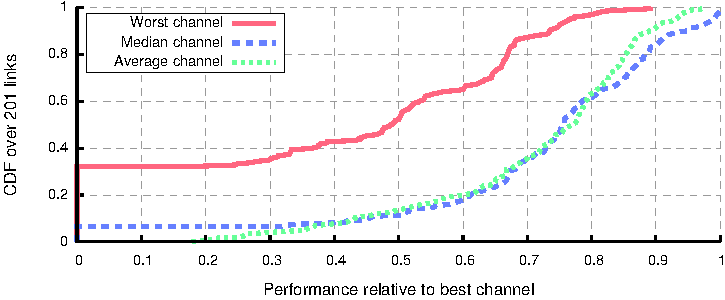
\includegraphics[width=\textwidth]{figures/applications/chan_sel_rel_diff.pdf}
	\caption{\label{fig:chan_sel_rel_diff}The relative difference in throughput over 802.11n channels.}
\end{figure}

\begin{figure}[t]
	\centering
	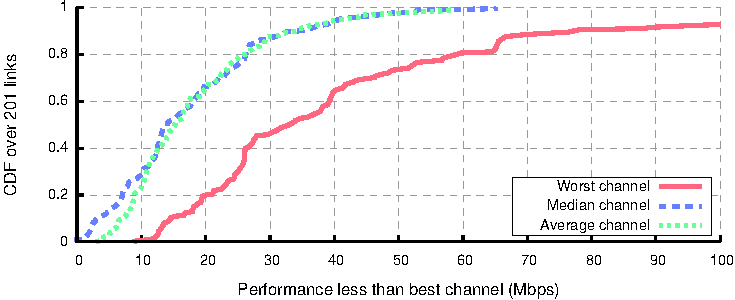
\includegraphics[width=\textwidth]{figures/applications/chan_sel_tpt_diff.pdf}
	\caption{\label{fig:chan_sel_tpt_diff}The absolute difference in throughput over 802.11n channels.}
\end{figure}

\figref{fig:chan_sel_rel_diff} and \figref{fig:chan_sel_tpt_diff} show how the throughput of the worst, median, and average channels compares to the best channel for these links. Note that because the channel set is fixed and independent of connectivity, the worst channel might deliver no throughput at all---unlike AP selection, in which the client was choosing from only those nodes that responded to its probe. About a third of the links had at least one such channel.

These figures demonstrate that the choice of channel can dramatically impact performance. \figref{fig:chan_sel_rel_diff} shows that the worst channel offers less than half of the best throughput for more than half the links. In absolute terms, this difference can be quite large: the worst channel is a median 33\Mbps worse than the best channel, and for a few links (about 7\%) the difference is more than 100\Mbps. For these links, some channel will deliver no packets at all, while another delivers packets at nearly the maximum bitrate. An unlucky choice of channel can cripple performance and result in little to no throughput.

The median and average channels perform about equivalently in our testbed, and even these are significantly worse. These channels yield less than half the optimal throughput for 15\% of the links and for only one third of links do these come within 80\% of the best throughput. These figures show that for very few links do most channels perform about the same, and the median or average channel is 15\Mbps worse than the best channel for most links, and the gap is larger than 25\Mbps for 20\% of links.

Note that in these graphs, the average/median channels are much closer to optimal than are the average/median access points we saw in \figref{fig:ap_sel_rel_diff} and \figref{ap_sel_tpt_diff}. I hypothesized that this might be because different channels between the same two devices are likely to have similar total signal strengths (i.e., Packet SNR). If this is the case, the difference in performance will come mainly through subchannel fading effects---and while these subchannel effects can affect link quality significantly, as I showed in \chapref{chap:delivery}, the difference is likely not as much as when comparing access points located tens of meters apart.

To test this hypothesis, I analyzed the Packet SNR versus channel for the 11 channels supported by the IWL5300 in the 2.4\GHz band and the 24 channels in the 5\GHz band. Note that for these experiments, external interference does not pose a problem because accurate SNR measurements require only a single packet to be delivered successfully without interference during the preamble. I considered only links that had at least 10 packets delivered with consistent SNRs and supported at least 3 channels, for a total or 349 links in the 2.4\GHz band and 253 links in the 5\GHz band. \figref{fig:rssi_vs_freq_24} and \figref{fig:rssi_vs_freq_5} plots the normalized Packet SNR (Packet SNR across all channels minus the average Packet SNR) against channel for these links. The figures include one grey line per link, and the solid black line in each figure shows the median. We see that, indeed, Packet SNR stays within a few dB of the median for most channels. I believe that the shape of the black line in \figref{fig:rssi_vs_freq_5} shows the natural resonance of the antennas, which is consistently non-uniform across the approximately 600\MHz of spectrum the 5\GHz band covers.

\begin{figure}[htp]
	\centering
	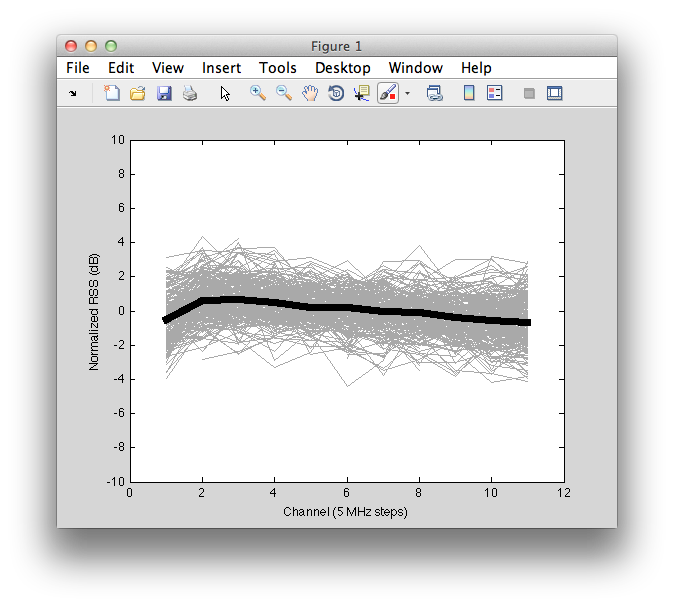
\includegraphics[width=0.6\textwidth]{figures/esnr/rssi_vs_freq_24.png}
	\caption{\label{fig:rssi_vs_freq_24}Normalized Packet SNR versus 2.4\GHz channel for 349 links. Solid line shows the median for each channel.}
\end{figure}
\begin{figure}[htp]
	\centering
	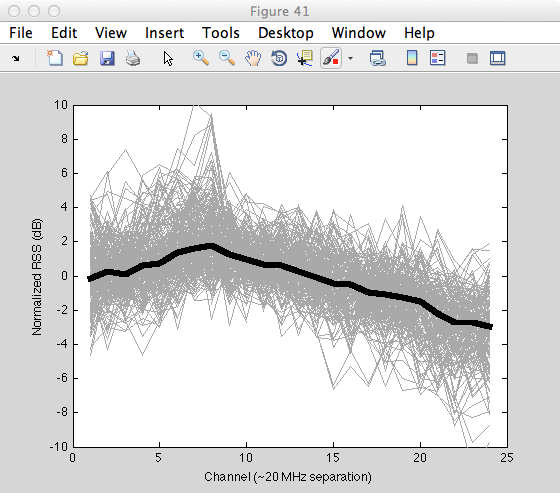
\includegraphics[width=0.6\textwidth]{figures/esnr/rssi_vs_freq_5.png}
	\caption{\label{fig:rssi_vs_freq_5}Normalized Packet SNR versus 5\GHz channel for 253 links. Solid line shows the median for each channel.}
\end{figure}
%\begin{figure}[htp]
%	\centering
%	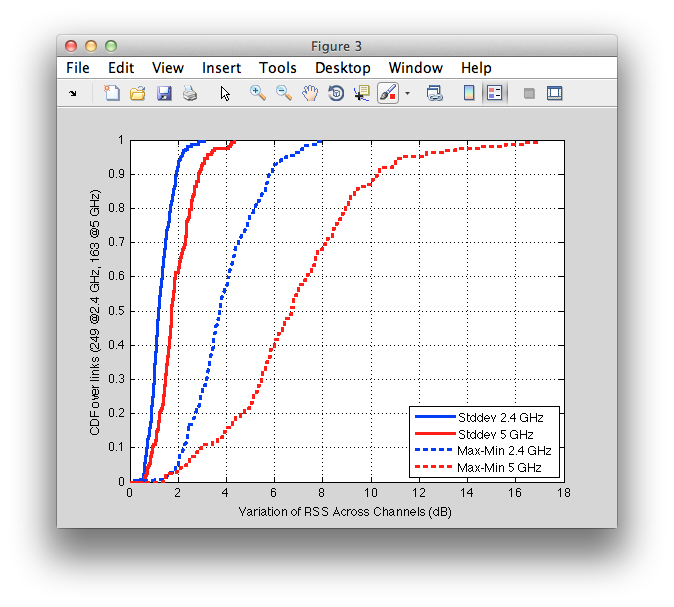
\includegraphics[width=0.6\textwidth]{figures/esnr/rssi_freq_dev.png}
%	\caption{\label{fig:rssi_freq_dev}Standard deviation and max-min spread of Packet SNR across channels within the same band.}
%\end{figure}

From these results, I conclude that a strategy that picks a fixed channel or a random channel will perform significantly worse than a strategy that can identify channels that are likely to offer good performance. Note that this is implicitly the channel selection strategy for strategies that attempt to short-circuit the AP~\cite{Afanasyev_RTSid} used in today's infrastructure networks, because the channel is fixed by the AP. At the same time, because for a fixed link, most channels have roughly the same Packet SNR, fading effects should play a larger role in determining the best channel. This makes the channel selection problem is harder than the AP selection problem, and the solutions may perform slightly worse; however Effective SNR should provide a larger advantage in this case. Having motivated the need for an accurate channel selection algorithm, I present and evaluate different channel selection strategies in the rest of this section.

%%%%%%%%%%%%%%%%%%%%%%%%%%%%%%%%%%%%%%%%%%%%%%%%%%%%%%%%%%%%%%%%%%%%%%%%%%%%%%%%%%%%%%%%%%%%%%%%%%%%%%%%%%%%%%%%%%%%%%%%%%%%%%%%%%%%%%%%%%
%\subsection{Channel selection algorithms}
%\algref{alg:chan_sel_basic} is a template for a channel selection algorithm. It takes as input a list of channels to evaluate $C$, and a sender $s$ and receiver $r$ that together define a link. The two nodes hop across channels, using the \fcall{PredictThroughput} function to evaluate the performance of the link on each. The algorithm tracks the best performing channel, labeled $c_{\max}$ and returns that value. (\fcall{ChannelSelection} can also return $\emptyset$ if all channels have zero predicted throughput, but we only consider links that can communicate on at least 1 channel.) Using this template, different channel selection algorithms can be instantiated by providing different implementations of \fcall{PredictThroughput}.
%
%%%%%%%%%%%%%%%%%%%%%%%%%%%%%%%%%%%%%%%%%%%%%%%%%
%\begin{algorithm}[htp]
%\caption{\label{alg:chan_sel_basic}\fcall{ChannelSelection($C, s, r$)}}
%\begin{algorithmic}
%\STATE $t_{\max}\gets 0\Mbps$
%\STATE $c_{\text{best}} \gets \emptyset$
%\FORALL{$c \in C$}
%\STATE Both $s$ and $r$ switch to channel $c$
%\STATE $t \gets \fcall{PredictThroughput($s, r$)}$
%\IF{$t > t_{\max}$}
%	\STATE $t_{\max} \gets t$
%	\STATE $c_{\text{best}} \gets c$
%\ENDIF
%\STATE \textbf{return} $c_{\text{best}}$
%\ENDFOR
%\end{algorithmic}
%\end{algorithm}
%%%%%%%%%%%%%%%%%%%%%%%%%%%%%%%%%%%%%%%%%%%%%%%%%
%
%I consider three different channel selection algorithms in this section. The first is \fcall{ChannelSelectionOPT}, an oracular channel selection algorithm that chooses the optimal channel. For implementation purposes, I instantiate \fcall{ChannelSelectionOPT} by \algref{alg:chan_sel_probe} (\fcall{ProbeChannelThroughput}), which probes all MCSes with MTU-sized packets to determine packet delivery and predicts throughput according to \eqref{eq:prr_throughput}.
%
%%%%%%%%%%%%%%%%%%%%%%%%%%%%%%%%%%%%%%%%%%%%%%%%%
%\begin{algorithm}[tp]
%\caption{\label{alg:chan_sel_probe}\fcall{ProbeThroughput($s, r$)}}
%\begin{algorithmic}
%\STATE $p_0,p_1,\dots,p_{23} \gets 0$
%\STATE $N \gets \text{number of probes at each MCS}$
%\FOR{$i = 1 \dots N$}
%\FOR{$m = 0 \dots 23$}
%\STATE $s$ sends one MTU-sized packet at \mcs{$m$}
%\IF{$s$ receives an ACK from $r$}
%\STATE $p_m \gets p_m + 1$
%\ENDIF
%\ENDFOR
%\ENDFOR
%\STATE $t_{\max}\gets \max \{p_m/N \cdot M(m)\} \text{ over all } m$ \hfill \COMMENT{\eqref{eq:prr_throughput}}
%\STATE \textbf{return} $t_{\max}$
%\end{algorithmic}
%\end{algorithm}
%%%%%%%%%%%%%%%%%%%%%%%%%%%%%%%%%%%%%%%%%%%%%%%%%
%%%%%%%%%%%%%%%%%%%%%%%%%%%%%%%%%%%%%%%%%%%%%%%%%
%\begin{algorithm}[tp]
%\caption{\label{alg:chan_sel_esnr}\fcall{PredictThroughputESNR($s, r$)}}
%\begin{algorithmic}
%\FOR{$m \in \{16, 8, 0\}$}
%\STATE $s$ sends one packet with 0-byte payload at \mcs{$m$}
%\STATE $r$ computes the Effective SNR values $\rho_\text{eff}$ and returns them along with the ACK
%\IF{$s$ receives an ACK from $r$}
%	\STATE \textbf{return} \fcall{ESNRToThroughput}($\rho_\text{eff}$), $\rho_\text{eff}$ \hfill \COMMENT{$\rho_\text{eff}$ is used to break ties}
%\ENDIF
%\ENDFOR
%\STATE \textbf{return} 0
%\end{algorithmic}
%\end{algorithm}
%%%%%%%%%%%%%%%%%%%%%%%%%%%%%%%%%%%%%%%%%%%%%%%%%
%
%The second algorithm chooses the channel based on RSS, presented in \algref{alg:chan_sel_rss}. In this case, the sender only needs to send a single probe packet (with no payload) in order to measure the RSS on the channel. Since \fcall{RSSToThroughput} is monotonically increasing in RSS, this algorithm is equivalent to selecting the channel with the maximum RSS\@.
%
%The third algorithm chooses the channel based on the Effective SNR, presented in \algref{alg:chan_sel_esnr}. Here, the sender sends probes (with no payload) with decreasing numbers of spatial streams to enable the receiver to collect a maximal CSI measurement. The receiver then sends the computed Effective SNR values back to the sender, which uses them to predict the best rate.
%
%I evaluate these three algorithms in the next section.

%%%%%%%%%%%%%%%%%%%%%%%%%%%%%%%%%%%%%%%%%%%%%%%%%%%%%%%%%%%%%%%%%%%%%%%%%%%%%%%%%%%%%%%%%%%%%%%%%%%%%%%%%%%%%%%%%%%%%%%%%%%%%%%%%%%%%%%%%
\subsection{Channel selection accuracy}
I evaluate Packet SNR and Effective SNR-based channel selection algorithms bases on \algref{alg:chan_sel_basic} and using the link metric functions described in \algref{alg:snr_link_metric} (Packet SNR) and \algref{alg:eff_snr_link_metric} (Effective SNR).

\figref{fig:chan_sel_ratio_opt} shows the performance relative to the optimal algorithm when using Effective SNR or Packet SNR to choose between channels, using the same format as I used for access point selection in \figref{fig:ap_sel_ratio_opt}. Again, we see that both algorithms perform well, though Effective SNR is a better predictor of application performance. Note that the accuracy of both algorithms is reduced relative to access point selection, as hypothesized above. Whereas Effective SNR chose an optimal AP for more than 80\% of clients, it finds an optimal channel for only 60\% of links; the Packet SNR results exhibit similar a similar decline. This confirms that the similarity of channels leads to more ambiguity when choosing between them.

In this figure, Effective SNR chooses an optimal channel for 121 links (60\%), whereas Packet SNR is optimal for only 73 links (36\%). The Effective SNR-based algorithm is within 90\% of optimal for 168 links (84\%), 80\% for 181 links (90\%), and 70\% for 191 links (95\%). In contrast, maximizing the Packet SNR only gets within 90\% of optimal for 123 links (61\%).

\begin{figure}[p]
	\centering
	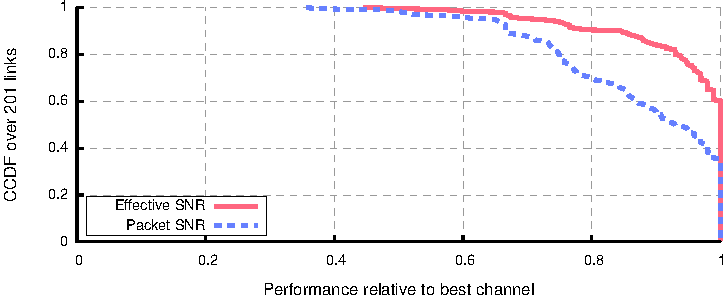
\includegraphics[width=\textwidth]{figures/applications/chan_sel_ratio_opt.pdf}
	\caption{\label{fig:chan_sel_ratio_opt}Channel selection algorithm performance relative to an optimal algorithm.}
\end{figure}
\begin{figure}[p]
	\centering
	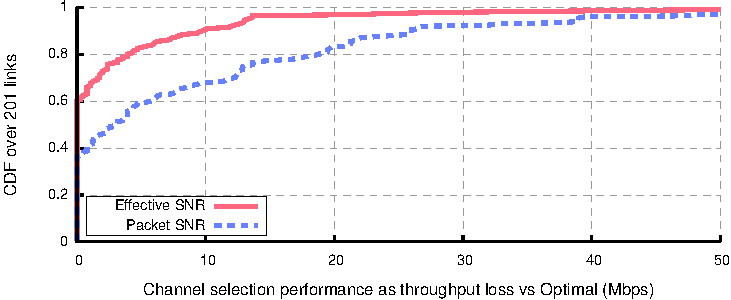
\includegraphics[width=\textwidth]{figures/applications/chan_sel_diff_opt.pdf}
	\caption{\label{fig:chan_sel_delta_opt}Channel selection algorithm performance loss from optimal algorithm.}
\end{figure}
\begin{figure}[p]
	\centering
	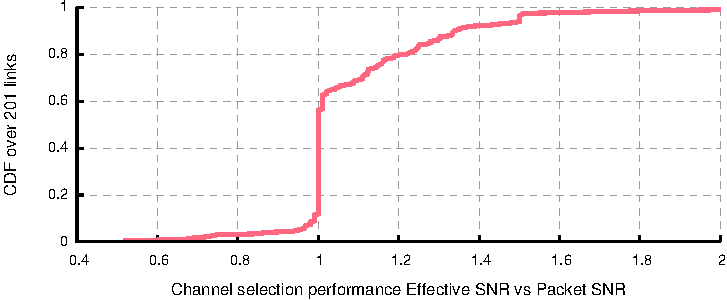
\includegraphics[width=\textwidth]{figures/applications/chan_sel_ratio.pdf}
	\caption{\label{fig:chan_sel_ratio}Channel selection performance with Effective SNR relative to RSS\@.}
\end{figure}

Next, I compare the absolute performance loss of the channel selection algorithms in \figref{fig:chan_sel_delta_opt}. Here, each $(x,y)$ point represents the fraction of links $y$ that choose a channel within $y$\Mbps of the best channel with a particular algorithm. The area over the curves represents the performance lost by each algorithm; an accurate algorithm would be in the top left corner, losing little throughput for only a few links. This area is 2.9$\times$ larger for the Packet SNR-based selection algorithm, showing that Effective SNR is significantly more accurate. This difference translates to about 10\Mbps more per link when selecting channels via the Effective SNR\@.

Finally, I examine the head-to-head performance of selecting channels via Effective SNR or Packet SNR in \figref{fig:chan_sel_ratio}. For each link, I plot the ratio of the performance of the channel picked with the Effective SNR strategy to that of the channel chosen by maximizing Packet SNR. If the two channels perform equally, the ratio will be 1; if the Effective SNR strategy chose a better channel the ratio will be larger. The algorithms choose channels with equal performance for 90 (45\%) of the 201 links, while the Effective SNR-based algorithm chooses a better channel for 88 (44\%) links and the Packet SNR-based algorithm for the remaining 23 (11\%). Additionally, the gains from Effective SNR are much larger than its losses: the Packet SNR strategy chooses a channel that performs 20\% better than the Effective SNR-selected channel for only 6/23 (26\%) links its channel is better, while Effective SNR chooses a 20\% better channel for 41/88 (47\%) of cases. In other words, the Effective SNR channel selection algorithm is more likely to pick a better channel by a factor of about 4 (88/23), and this difference is more likely to be significant by a factor of about 2 (47\%/26\%).

In conclusion, these results shows that both Effective SNR- and Packet SNR-based channel selection strategies perform well in my testbed. However, the Effective SNR channel selection strategy is significantly more accurate: it chooses an optimal channel for 66\% more links, it offers about 10\Mbps more per link when selecting suboptimal channels, and it is more likely to choose a better channel by a factor of 4.

%%%%%%%%%%%%%%%%%%%%%%%%%%%%%%%%%%%%%%
\subsubsection{Channel discrimination}
\xxx{how many channels do we need to look at to get good performance?} \figref{fig:rel_diff_draws} shows that, depending on how close to optimal you want to be, need to look at 5, 10, or 15 of the 24 channels in 5\GHz band. If we can evaluate the rate offered by a channel quickly, we can look at more channels in the same amount of time to pick the best rate.

\begin{figure}[htp]
	\centering
	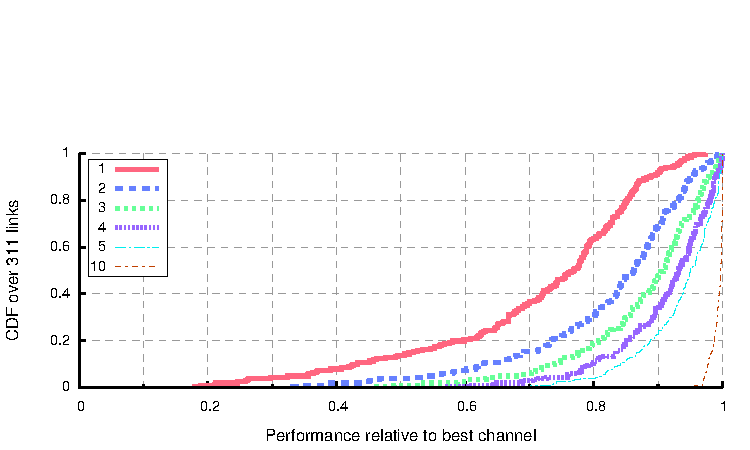
\includegraphics[width=\textwidth]{figures/applications/chan_sel_rel_diff_draws.pdf}
	\caption{\label{fig:rel_diff_draws}The expected rate after choosing the best of $k$ 802.11n channels.}
\end{figure}

\xxx{idea: maybe we can tell whether we're on a ``good'' channel by comparing Effective SNR to Packet SNR---the difference captures some notion of inefficiency. This might let us get good performance by checking just enough channels to determine we found a good one, rather than checking them all or a uniform constant fraction of them all.}

%%%%%%%%%%%%%%%%%%%%%%%%%%%%%%%%%%%%%%%%%%%%%%%%%%%%%%%%%%%%%%%%%%%%%%%%%%%%%%%%%%%%%%%%%%%%%%%%%%%%%%%%%%%%%%%%%%%%%%%%%%%%%%%%%%%%%%%%%
\subsection{Further Evaluations?}
\heading{Performance.}  given time to hop $\mathcal{O}$(1\ms), time to execute a CSI probe $\mathcal{O}$(500\us), and time to execute a rate probe (unknown), how many channels can we look at in $T$ time? Reference \figref{fig:rel_diff_draws} to see what fraction of optimal this enables.

\heading{Completion Time.} The difference between the Effective SNR and the SNR is a proxy for how ``good'' a channel is, based on how flat it is. Given that RSS is similar across channels, the flattest channel will likely offer the best rate. Can we use this to detect a good channel and stop looking early?